\documentclass[12pt]{article}
\usepackage[utf8]{inputenc}

\usepackage{mathptmx}

\usepackage{amsmath}
\usepackage{amsthm}
\usepackage{amsfonts}
%\usepackage{amscd}
\usepackage{amssymb}
\usepackage{graphicx}
\usepackage{mathtools}
\usepackage{natbib}
\usepackage{url}
\usepackage{bm}

\usepackage{geometry}
\usepackage[usenames]{color}
\geometry{margin=1in}

\newcommand{\R}{\mathbb{R}}
\newcommand{\Y}{\mathcal{Y}}
\newcommand{\X}{\mathcal{X}}
\newcommand{\Hcal}{\mathcal{H}}

\newcommand{\Ybf}{\textbf{Y}}
\newcommand{\Xbf}{\textbf{X}}
\newcommand{\Hbf}{\textbf{H}}
\newcommand{\Pbf}{\textbf{P}}
\newcommand{\V}{\textbf{V}}
\newcommand{\W}{\textbf{W}}
\newcommand{\y}{\textbf{y}}
\newcommand{\x}{\textbf{x}}
\newcommand{\h}{\textbf{h}}
\newcommand{\w}{\textbf{w}}
\newcommand{\s}{\textbf{s}}
\newcommand{\tbf}{\textbf{t}}
\newcommand{\Wstar}{\W^{\textstyle{*}}}
\newcommand{\wstar}{w^{\textstyle{*}}}
\newcommand{\wstarsq}{w^{\textstyle{*}^2}}
\newcommand{\wstarpwr}{w^{\textstyle{*}^{5/4}}}
\newcommand{\lamstar}{\lambda^{\textstyle{*}}}
\newcommand{\lambdabf}{\boldsymbol{\lambda}}

\newcommand{\norm}[1]{\left\lVert#1\right\rVert}
\newcommand{\indep}{\perp\!\!\!\perp}

\DeclareMathOperator{\E}{E}
\DeclareMathOperator{\Var}{Var}
\DeclareMathOperator{\MSE}{MSE}


\newtheorem{cor}{Corollary}
\newtheorem{lem}{Lemma}
\newtheorem{thm}{Theorem}
\newtheorem{defn}{Definition}
\newtheorem{prop}{Proposition}

\newcommand\red[1]{{\color{red}#1}}

\allowdisplaybreaks

\title{SEAM methodology for context-rich player matchup evaluations in baseball}
%\author{Charles Young\thanks{cdy2@illinois.edu}, 
%David Dalpiaz\thanks{dalpiaz2@illinois.edu}, 
%and Daniel J. Eck\thanks{dje13@illinois.edu} \\[1em]
%Department of Statistics, University of Illinois Urbana-Champaign
%}
\date{}

\linespread{2}

\begin{document}

\maketitle

\begin{abstract}
We develop SEAM (synthetic estimated average matchup) methodology which can be used to evaluate batter versus pitcher matchups, both numerically and visually. We first estimate the distribution of balls put into play by a batter facing a pitcher, called the spray chart distribution. This distribution is conditional on batter and pitcher characteristics. These characteristics are a better expression of talent than any conventional statistics. Many individual matchups have a sample size that is too small to be reliable. Synthetic versions of the batter and pitcher under consideration are constructed in order to alleviate these concerns. Weights governing how much influence these synthetic players have on the overall spray chart distribution are constructed to minimize expected mean square error. We provide novel performance metrics that are calculated as expectations taken with respect to the spray chart distribution. These performance metrics provide a context rich approach to player evaluation. We also provide a Shiny app that allows users to visualize and evaluate any batter-pitcher matchup that has occurred or could have occurred in the last five years. One can access this app at \url{https://seam.shinyapps.io/seam/}. Our methodology and interactive tool has utility for anyone interested in baseball as well as team executives and players.
\end{abstract}

\noindent\textbf{Keywords}: Nonparametric density estimation; Similarity scores; Model averaging; Reproducible research; Sabermetrics; Big data applications and visualization


\section{Introduction}

Baseball has a rich statistical history dating back to the first box score created by Henry Chadwick in 1859. Fans, journalists, and teams have obsessed over baseball statistics and performance metrics ever since. This passion for baseball statistics is best summarized by the existence of \cite{schwarz2004numbers}, a best selling book devoted entirely to the statistical history of baseball. Baseball data is analyzed in the classroom as well. Max Marchi, Jim Albert, and Benjamin S. Baumer have written a book that teaches R through baseball analysis \citep{marchi2019analyzing}, and Jim Albert maintains an actively updated website Exploring Baseball Data with R that supplements this book. 
Quantification of players' skill has appeared in the Statistics literature, with articles devoted to
hitting \citep{berry1999bridging, albert2008streaky, brown2008season, jensen2009hierarchical},
pitching \citep{albert2006pitching, shinya2017pitching},
fielding \citep{jensen2009bayesball, piette2012estimating}, 
and total value \citep{baumer2015openwar}.


Most baseball statistics used for player evaluations are obtained from raw box score totals. While box score totals are an enjoyable statistical summary for baseball fans and analysts, the information contained in them is not very substantive. They ignore rich contextual information such as era, opposing team strength, and individual level matchup effects. Most commonly used player evaluation metrics are functions of context-free box score totals. These include, and are far from limited to, adjusted earned run average (ERA+), adjusted on base plus slugging percentage (OPS+), weighted runs created plus (wRC+), and wins above replacement (WAR) \citep{bref, fangraphs}. More sophisticated techniques in \citet{berry1999bridging}, \citet{brown2008season}, \cite{jensen2009hierarchical}, and \cite{baumer2015openwar} also constructed methodology grounded in raw box score totals. While many of these tools account for some contextual information such as ball parks, position of a player, and a player's age, they ignore opponent strength. %These metrics all ignore which pitchers a batter faced and the game situations which complement the outcomes that are recorded. 
\cite{eck2020challenging} showed that context-free metrics and the class of metrics that compares a player's accomplishments directly with that player's peers are ill-equipped for player comparisons across eras of baseball, although they may perform well over the course of a single season or a few consecutive seasons. That being said, these context-free metrics do not offer any guidance for how any particular batter will perform against a particular pitcher, the most important and relevant outcome in baseball. Furthermore, baseball outcomes have been assumed to be independent and identically distributed (iid) realizations in the literature \citep{brown2008season, jensen2009hierarchical}. The iid assumption of outcomes may be reasonable in the prediction contexts of \cite{brown2008season} and \cite{jensen2009hierarchical} that involve long time frames, but this assumption is not appropriate for small time frames when the variability in quality of batter and pitcher characteristics can be very large.



%Discuss how PECOTA, \cite{jensen2009hierarchical}, \cite[Section 2.5]{jensen2009bayesball} pool players 

%The i.i.d. assumption underlying the binomial model has already been justified for hitting totals within a single season (Brown 2008), and so seems reasonable for hitting totals across an entire season. \citep[Section 2.1]{jensen2009hierarchical}. 
%
%Get: 
%Brown, L. D. (2008). “In-Season Prediction of Batting Averages: A Field-test of Simple Empirical Bayes and Bayes Methodologies.” Annals of Applied Statistics, 2: 113–152. 632, 633


In this article we develop SEAM methodology that can be used to evaluate batter-pitcher matchups visually and numerically. This methodology is built upon spray chart distributions which are 2-dimensional spatial distributions representing the potential batted-ball locations when a particular batter faces off against a particular pitcher. Spray chart distributions provide contours that overlay traditional spray charts \citep{pettispray, marchi2019analyzing}. We construct spray chart distributions for batter-pitcher matchups where separate batter spray chart distributions are constructed for each of the pitches that the pitcher throws. Rich pitch characteristic information is used to supplement labelled pitch type data since the velocity, trajectory, movement characteristics, and release points of a pitch exhibit large variation across pitchers. The reported spray chart distribution for the batter pitcher matchup is the aggregation of the spray chart distributions for each pitch that the pitcher throws. The aggregation is with respect to the percentage that the pitcher throws each pitch. The density functions corresponding to these spray chart distributions are estimated nonparametrically using the \texttt{kde2d} function in the \texttt{MASS} R package \citep{MASS}.
%We can use spray distributions to calculate player evaluation metrics directly from batted ball location data instead of from outcomes that are obtained from the boxscore. We also motivate a synthetic player construction that can lead to estimated spray chart distributions with lower mean squared error (MSE).

One concern with the use of spray chart distributions is the potential sparsity of batter-pitcher matchup data. We alleviate this concern through the development and aggregation of synthetic batters and pitchers with similar characteristics as the batter and pitcher under study. Our synthetic player creation methodology is inspired by the notion of similarity scores \citep{james1994politics, PECOTA}. However, unlike the similarity scores presented in \cite{james1994politics} and \cite{PECOTA}, we construct similarity scores using a nearest neighbor approach that is based on the underlying batter and pitcher characteristics of the players under study instead of observed statistics. The pitcher characteristics that we consider are averages of the velocity, trajectory, movement, and release point of pitches thrown. The batter characteristics that we consider are averages of launch angle, exit velocity, spray angle, and binned batted ball location information. These player characteristics are obtained from Statcast \citep{statcast} scraped using functionality in the \texttt{baseballr} R package \citep{baseballr}, and reflect the underlying talent and tendencies of players. For each batter-pitcher matchup we estimate three spray chart densities, the first is the natural spray chart density corresponding to the players under study, the second is the spray chart of the synthetic pitcher versus the original batter, and the third is the spray chart of the original pitcher versus the synthetic batter. We report a synthetic spray chart density which is a weighted average of these spray chart densities where the weights are chosen with the aim of minimizing mean squared error. 

We also provide a Shiny app which gives users the ability to display the synthetic spray chart distribution for any batter pitcher matchup that has occurred or could have occurred in the last five years, the years that Statcast data exists. These synthetic spray charts are visualized over an image of a representative baseball field so that this spray chart distribution is displayed to give proper context. We also report performance metrics that are computed as expectations with respect to the synthetic spray chart distribution. The expected number of singles, doubles, triples, home runs are reported. The expected batting average on balls in play (xBABIP) and the expected bases on contact (xBsCON) are also reported. These matchup dependent metrics allow for any user to assess the expected performance of batters and pitchers when they face each other. 




\section{Spray chart distributions and densities}

A spray chart distribution for a batter is a distribution $F$ over a bounded subset $\Y \in \R^2$. The set $\Y$ contains plausible locations of batted balls from home plate. Let $(0,0) \in \Y$ denote the location of home plate. With this specification we can take $\Y = \{\y \in \R^2: \|\y\| \leq 1000\}$ where values in $\Y$ are locations in feet and $\|\cdot\|$ is the Euclidean norm. This specification of $\Y$ guarantees that $F(\Y) = 1$ for all batters in history. No human in history has ever come close to hitting a ball 1000 feet.


Let $f$ be the spray chart density function corresponding to the spray chart distribution $F$ for the matchup between a particular pitcher and a particular batter. Let $(y_{1i},y_{2i}) \in \Y$, $i = 1, \ldots, n$, be the observed batted-ball locations for this matchup. We will estimate $f$ with a multivariate kernel density estimator
\begin{equation} \label{general}
  \hat f_\Hbf(\y) = \frac{1}{n|\Hbf|}\sum_{i=1}^{n} K\left(\Hbf^{-1}(\y_i - \y)\right), 
  \qquad \y \in \Y, 
\end{equation}
where $K$ is a multivariate kernel function and $\Hbf$ is a matrix of bandwidth parameters. Our implementation will estimate $f$ using the \texttt{kde2d} and \texttt{kde2d.weighted} functions in R \citep{MASS, ggtern}. These functions are chosen because of their presence in the \texttt{ggplot2} R package \citep{ggplot2} which will be employed for visualization. Therefore, we estimate $f$ using a bivariate nonparametric Gaussian kernel density estimator
\begin{equation} \label{spraydens}
  \hat f_\h(\y) = 
    \frac{1}{n h_{y_1}h_{y_2}}\sum_{i=1}^{n} \phi\left(\frac{y_1 - y_{1i}}{h_{y_1}}\right)
      \phi\left(\frac{y_2 - y_{2i}}{h_{y_2}}\right),
\end{equation}
where $\y = (y_1, y_2) \in \Y$, $\phi$ is a standard Gaussian density, $\h \in \R^2$ is a bandwidth parameter so that the matrix $\Hbf$ in \eqref{general} is $\Hbf = \text{diag}(\h)$, and $\Hbf$ is chosen according to the default bandwidth selection procedures within the \texttt{kde2d} and \texttt{kde2d.weighted} functions. The estimated spray chart density function $\hat f_\h$ is a smoothed surface overlaying a spray chart. Our visualization of the spray chart distribution will be along $n_g$ common grid points $g_1,\ldots,g_{n_g}$ for all matchups under study. Commonality of grid points allows for straightforward comparisons of spray chart distributions in practice.




We extend this framework to spray chart distributions that are conditional on several characteristics for pitchers $\x_p$ and batters $\x_b$, where $\x = (\x_p',\x_b')' \in \X$, and $\X$ is assumed to be bounded. Denote the conditional spray chart distribution as $F(\y|\x)$ for $\x \in \X$ and $\y \in \Y$. The conditional spray chart density function corresponding to $F(\y|\x)$ will be denoted as $f(\y|\x)$ for all $\x \in \X$ and $\y \in \Y$. Thus, $f(\y|\x)$ is a nonparametric regression model that we will again estimate with a bivariate nonparametric Gaussian kernel density estimator
\begin{equation} \label{spraydens-cov}
  \hat f_\h(\y|\x) = 
    \frac{1}{n h_{y_1}h_{y_2}}\sum_{i=1}^{n} \phi\left(\frac{y_1 - y_{1i}}{h_{y_1}}\right)
      \phi\left(\frac{y_2 - y_{2i}}{h_{y_2}}\right),
\end{equation}
where the sample of batted-ball locations $(y_{1i},y_{2i}) \in \Y$, $i = 1, \ldots, n$ are now conditional on $\x \in \X$.


\subsection{Synthetic player construction}

We develop a method for synthetically recreating baseball players in order to alleviate the small sample size concerns inherent in the estimation of $f$ for any batter-pitcher matchup. Matchup data involving these synthetic players will then be included in our analysis to estimate $f$. We first develop the similarity scores used in this methodology. We will suppose that there are $J$ pitchers and $K$ batters available in our donor pool. We will suppose that the pitcher in the matchup under study throws $n_{\text{pitch types}}$ different types of pitches. We will let $\x_p^t$ be the pitcher covariates for pitch type $t = 1,\ldots,n_{\text{pitch types}}$. We will denote $d_p$ and $d_b$ as the dimensions of $\x_p^t$ and $\x_b$ respectively. For a pitch type $t$, the similarity score of pitcher $j_1$ to pitcher $j_2$ is defined as $s(\x_{p,j_1}^t, \x_{p,j_2}^t) = \exp(-\|\x_{p,j_1}^t-\x_{p,j_2}^t\|_{\V_p})$ where $\x_{p,j_1}^t$ and $\x_{p,j_2}^t$ are, respectively, the underlying pitch characteristics for pitcher $j_1$ and $j_2$,
$$
   \|\x_{p,j_1}^t-\x_{p,j_2}^t\|_{\V_p} 
     = \left((\x_{p,j_1}^t-\x_{p,j_2}^t)'\V_p^t(\x_{p,j_1}^t-\x_{p,j_2}^t)\right)^{1/d_p},
$$ 
and $\V_p^t$ is a diagonal weight matrix that is chosen to scale the pitch characteristics and give preference to pitch characteristics that are chosen to have higher influence on the spray chart distribution under study. Similarity scores of the form $s(\x_{p,j_1}^t, \x_{p,j_2}^t)$ have desirable theoretical properties that are explained in the appendix and, in practice, they guard against downplaying the effect of the players under study. The user of our Shiny app has some control of the entries of $\V_p^t$ by adjusting the pitcher slider. Similarity scores for batters $s(\x_{b,k_1}, \x_{b,k_2})$, $1 \leq k_1,k_2 \leq K$ are defined in a similar manner. Implicit in this construction is the assumption that the underlying pitcher and batter characteristics that we collect are an exhaustive set of inputs to properly estimate the spray chart distribution.

We describe the synthetic spray chart density for the batter under study facing the synthetic version of the pitcher under study. Without loss of generality, let $\x_p^t$ be the characteristics for pitch type $t$ thrown by the pitcher under study, let $\x_b$ be the characteristics for the batter under study, and let $\x^t$ denote the vector of $x_p^t$ and $\x_b$. We then line up the pitcher characteristics for all of the pitchers in the donor pool, $\x_{p,j}^t$, $j = 1,...,J$. Now obtain the similarity scores $s_{p,j}^t = s(\x_p^t,\x_{p,j}^t)$ and then construct the weights $w_{p,j}^t = s_{p,j}^t / \sum_{l=1}^{J}s_{p,l}^t$, for $j = 1,...,J$. For pitch type $t$, the spray chart density for a batter facing the synthetic pitcher is 
\begin{equation} \label{synth-pitch-t}
  f_{\text{sp}}^t(\y|\x_b) = \sum_{j=1}^J w_{p,j}^tf(\y|\x_{p,j}^t,\x_b).
\end{equation}
Let $\rho_t$ be the proportion of time that the pitcher in the matchup under study throws pitch $t$, so that $\sum_t \rho_t = 1$. The spray chart density for a batter facing the synthetic pitcher is then
\begin{equation} \label{synth-pitch}
  f_{\text{sp}}(\y|\x_b) = \sum_{t=1}^{n_{\text{pitch types}}} \rho_t f_{\text{sp}}^t(\y|\x_b).
\end{equation}


We describe the synthetic spray chart density for the synthetic batter facing the pitcher under study. For pitch type $t$, we line up the batter characteristics for all of the available batters that faced pitch type $t$ thrown by the pitcher under study, $\x_{b,k}$, $k = 1,...,K^t$.  We obtain the similarity scores $s_{b,k}^t = s(\x_b,\x_{b,k})$ and then construct the weights $w_{b,k}^t = s_{b,k}^t / \sum_{l=1}^{K}s_{b,l}^t$, for $k = 1,...,K^t$. For pitch type $t$, the spray chart density for a pitcher facing the synthetic batter is 
\begin{equation} \label{synth-bat-t}
  f_{\text{sb}}^t(\y|\x_p^t) = \sum_{k=1}^K w_{b,k}^tf(\y|\x_p^t,\x_{b,k}).
\end{equation}
The spray chart density for the synthetic batter facing the pitcher under study is then
\begin{equation} \label{synth-bat}
  f_{\text{sb}}(\y) = \sum_{t=1}^{n_{\text{pitch types}}} \rho_t f_{\text{sb}}^t(\y|\x_p^t).
\end{equation}


We then estimate \eqref{synth-pitch-t} and \eqref{synth-bat-t} with
\begin{equation} \label{synth-est-t}
  \hat f_{\text{sp}}^t(\y|\x_b) = \sum_{j=1}^J w_{p,j}^t\hat f_{\h_{p,j}}(\y|\x_{p,j}^t,\x_b), 
  \qquad
  \hat f_{\text{sb}}^t(\y|\x_p^t) = \sum_{k=1}^K w_{b,k}^t\hat f_{\h_{b,k}}(\y|\x_p^t,\x_{b,k}),
\end{equation}
where, for pitch type $t$, we let $n_{p,j}^t$ denote the matchup sample size of pitcher $j$ versus the batter under study, $n_{b,k}^t$ denote the matchup sample size of the pitcher under study versus batter $k$, and $\h_{p,j}^t$ and $\h_{b,k}^t$ are bandwidth parameters. We estimate the densities in \eqref{synth-est-t} with,
\begin{equation} \label{synth-est}
  \hat f_{\text{sp}}(\y|\x_b) =  \sum_{t=1}^{n_{\text{pitch types}}} \rho_t \hat f_{\text{sp}}^t(\y|\x_b),
  \qquad
  \hat f_{\text{sb}}(\y) = \sum_{t=1}^{n_{\text{pitch types}}} \rho_t 
    \hat f_{\text{sb}}^t(\y|\x_p^t).
\end{equation}

Our implementation estimates the densities in \eqref{synth-est} with the \texttt{kde2d.weighted} function. The estimators \eqref{synth-est} are obviously biased estimators for $f$. However, they have the potential to reduce MSE. One obvious case is when, for all 
$t = 1,\ldots,n_{\text{pitch types}}$, there exists weights 
$w_{p,j}^t \approx 1$, $w_{b,k} \approx 1$ and 
$n_{p,j}^t > n$, $n_{b,k}^t > n$. 
In such settings, $f_{\text{sp}}(\y|\x_b)$ and $f_{\text{sp}}(\y|\x_b)$ have minimal bias when estimating $f$ and can be more efficient than $\hat f_h$. Another obvious case is when the batter has never faced the pitcher so that no data is available to estimate $f$ directly, although that does not guarantee that the estimators \eqref{synth-est} are good estimators for $f$. Our implementation will estimate $f$ with
\begin{equation} \label{sd-implem}
  \hat{g}_{\lambdabf}(\y|\x) = \lambda \hat f_\h(\y|\x) 
    + \lambda_p \hat f_{\text{sp}}(\y|\x_p) 
    + \lambda_b \hat f_{\text{sb}}(\y|\x_b)
\end{equation}
where $\lambda,\lambda_p$, $\lambda_b$ form a convex combination. %The choices of the elements of $\lambdabf$ will be discussed in the next Section where we calculate and compare the MSE of \eqref{spraydens} and \eqref{sd-implem}. 
Note that these calculations are conditional on the pitch characteristics which implies that they are also conditional on $w_{p,j}^t$ and $w_{b,k}^t$, $t = 1,\ldots,n_{\text{pitch types}}$, since the weights are a deterministic function of the pitch characteristics. Our implementation will estimate the elements of $\lambdabf$ as 
$$
  \lambda = \frac{\sqrt{n}}{\sqrt{n} + \sqrt{n_p} + \sqrt{n_b}}, \qquad
  \lambda_p = \frac{\sqrt{n_p}}{\sqrt{n} + \sqrt{n_p} + \sqrt{n_b}}, \qquad
  \lambda_b = \frac{\sqrt{n_b}}{\sqrt{n} + \sqrt{n_p} + \sqrt{n_b}},
$$
where $n_p = \sum_t\rho_t\sum_{j=1}^J (s_{p,j}^t)^2n_{p,j}^t$ and 
$n_b = \sum_t\rho_t\sum_{k=1}^K (s_{b,k}^t)^2n_{b,k}^t$.  These choices arise as a balance between the natural bias that exists in our synthetic player construction and the inherent estimation variation. %Denote $n^t$ as the number of times the batter under study put a ball in play when the pitcher under study threw pitch $t$. 
It is reasonable to assume that $n_{p,j}^t = O(n)$ and $n_{b,k}^t = O(n)$ for all $j = 1,\ldots,J$, all $k = 1,\ldots,K$, and all $t = 1,\ldots,n_{\text{pitch types}}$. It is also reasonable to assume that $n$ will be too small to be of much use, hence the reason why $n_p$ and $n_b$ are aggregated with respect to similarity scores instead of weights that form a convex combination. However, in the event that $n$ is large enough to provide reliable estimation of $f(\y|\x)$ with $\hat f_h(\y|\x)$, then $n$ dominates $n_p$ and $n_b$. Formal technical justification for selecting $\lambdabf$ is given in the Appendix. In the Appendix we argue that our choices of $\lambdabf$ lead to the estimator \eqref{sd-implem} having a lower MSE than the estimator \eqref{spraydens}.


\subsection{Performance metrics}

We develop novel performance metrics that are theoretically computed as expectations with respect to $\hat{g}_{\lambdabf}(\y|\x)$. We estimate the expected number of singles, doubles, triples, and home runs that the batter hits versus the pitcher in a particular matchup. We also estimate the xBABIP and xBsCON as additional summary measures. The metric xBsCON is best interpreted as slugging percentage conditional on balls put into play. Our implementation will not estimate these expectations exactly as there is not enough historical batted ball data.

To theoretically estimate these quantities we first obtain five years of batted ball data. We then estimate the proportion of batted balls that were either an out (O), single (1B), double (2B), triple (3B), or home run (HR) at locations $\y$ on the baseball field. Denote this vector of estimated proportions at $\y$ as 
$
  \widehat \Pbf(\y) =   
    \left(\hat p_\text{O}(\y),\hat p_{\text{1B}}(\y), \hat p_{\text{2B}}(\y),
      \hat p_{\text{3B}}(\y), \hat p_{\text{HR}}(\y)\right)'.
$ 
Next, we obtain $\widehat E(\x) = \int \Pbf(\y) \hat{g}_{\lambdabf}(\y|\x) d\y$, where 
$
  \widehat E(\x) 
    = (\hat e_{\text{O}}(\x), \hat e_{\text{1B}}(\x), \hat e_{\text{2B}}(\x), 
       \hat e_{\text{3B}}(\x), \hat e_{\text{HR}}(\x))'.
$
Thus $\widehat E(\x)$ is the estimated expected vector of outcomes where the expectation is taken with respect to the estimated spray chart distribution. 
Expected BABIP is then calculated as 
$
  \text{xBABIP} = \hat e_{\text{1B}}(\x) + \hat e_{\text{2B}}(\x) + \hat e_{\text{3B}}(\x)
$ 
and xBsCON is calculated as
$
  \text{xBsCON} = \hat e_{\text{1B}}(\x) + 2\hat e_{\text{2B}}(\x) 
    + 3\hat e_{\text{3B}}(\x) + 4\hat e_{\text{HR}}(\x).
$
Our Shiny app also displays the floor of $100 \hat e_{\text{1B}}(\x)$, $100 \hat e_{\text{2B}}(\x)$, $100 \hat e_{\text{3B}}(\x)$, and $100 \hat e_{\text{HR}}(\x)$. The 100 multiplier is a normalization that is intended for ease of interpretation. Note that there is not enough data available to estimate $\widehat \Pbf(\y)$ for every $\y \in \Y$. Therefore, we calculate discretized versions of these performance metrics over 10 feet by 10 feet bins.

\section{Data considerations}

Our methodology will consider the following variables comprising $\x_p$: velocity, spin rate, horizontal break, horizontal release angle, horizontal release point, vertical break, vertical release angle, vertical release point, and extension. Averages of these variables are taken across each pitcher-pitch type combination. Our methodology will consider the following variables comprising $\x_b$: exit velocity, launch angle, pull\%, middle\%, and oppo\%. Averages of these variables are taken across each batter-pitch type combination. One should note that these variables will not allow us to measure the complete talent profile of baseball players. %On average, players who hit the ball harder with a more optimized launch angle will receive better projected stats, since these balls tend to produce more home runs (and thus take fielders out of the equation). However, 
Tools such as speed and eye at the plate will not be fully captured by our methodology.

Data for our app was acquired via the \texttt{baseballr} R package \citep{baseballr}. This dataset contains every pitch thrown since 2015 that has been captured by Statcast. A few preprocessing steps are involved:
\begin{itemize}
    \item Pitches classified as Eephus, Knuckleball, and Screwball are removed since these pitch types are rare.
    \item Pitches classified as Knuckle-Curve are renamed to Curveball.
    \item Pitches classified as Forkball are renamed to Splitter.
    \item Pitch launch angles are calculated using rudimentary kinematics:
        \begin{itemize}
            \item $launch_h = \arctan(\frac{vx_r}{vy_r})$
            \item $launch_v = \arctan\left(\frac{vz_r}{\sqrt{vx_r^2 + vy_r^2}}\right)$
        \end{itemize}
        where $vx_r$, $vy_r$, $vz_r$ are, respectively, the $x$, $y$, $z$ components of release velocity.
    \item Batted ball locations are adjusted to reflect accurate baseball field coordinates \citep{petti2017research}.
    \item Spray angle is calculated from the x and y coordinates of the batted ball, and adjusted where a negative angle implies the ball was pulled.
    \item Player characteristic data are standardized to have mean zero and standard deviation 1. The player characteristic data are physically dimensionless after standardization. 
\end{itemize}

Pitchers are aggregated on a season and pitch type basis and batters are aggregated on a season, handedness, and pitch type basis. To be eligible for comparison, a pitcher must share at least  $\lceil \frac{n_{\text{pitch types}}}{2} \rceil$ pitches with the pitcher under study. 

 


\section{Shiny app}

In this section we present a snapshot of what our Shiny app implementing SEAM methodology offers users. The Shiny app is available at \url{https://seam.shinyapps.io/seam/}. The default matchup in the application pairs the reigning American League Cy Young winner Justin Verlander against the reigning American League MVP Mike Trout. The layout includes a sidebar with four filters: two dropdowns for batter/pitcher selection and two sliders for metric adjustment. A snapshot of the appearance of our visualization is depicted in Figures \ref{layout} and \ref{spraydists}.


\begin{figure}
\centering
\text{[Figure 1 about here]}
%    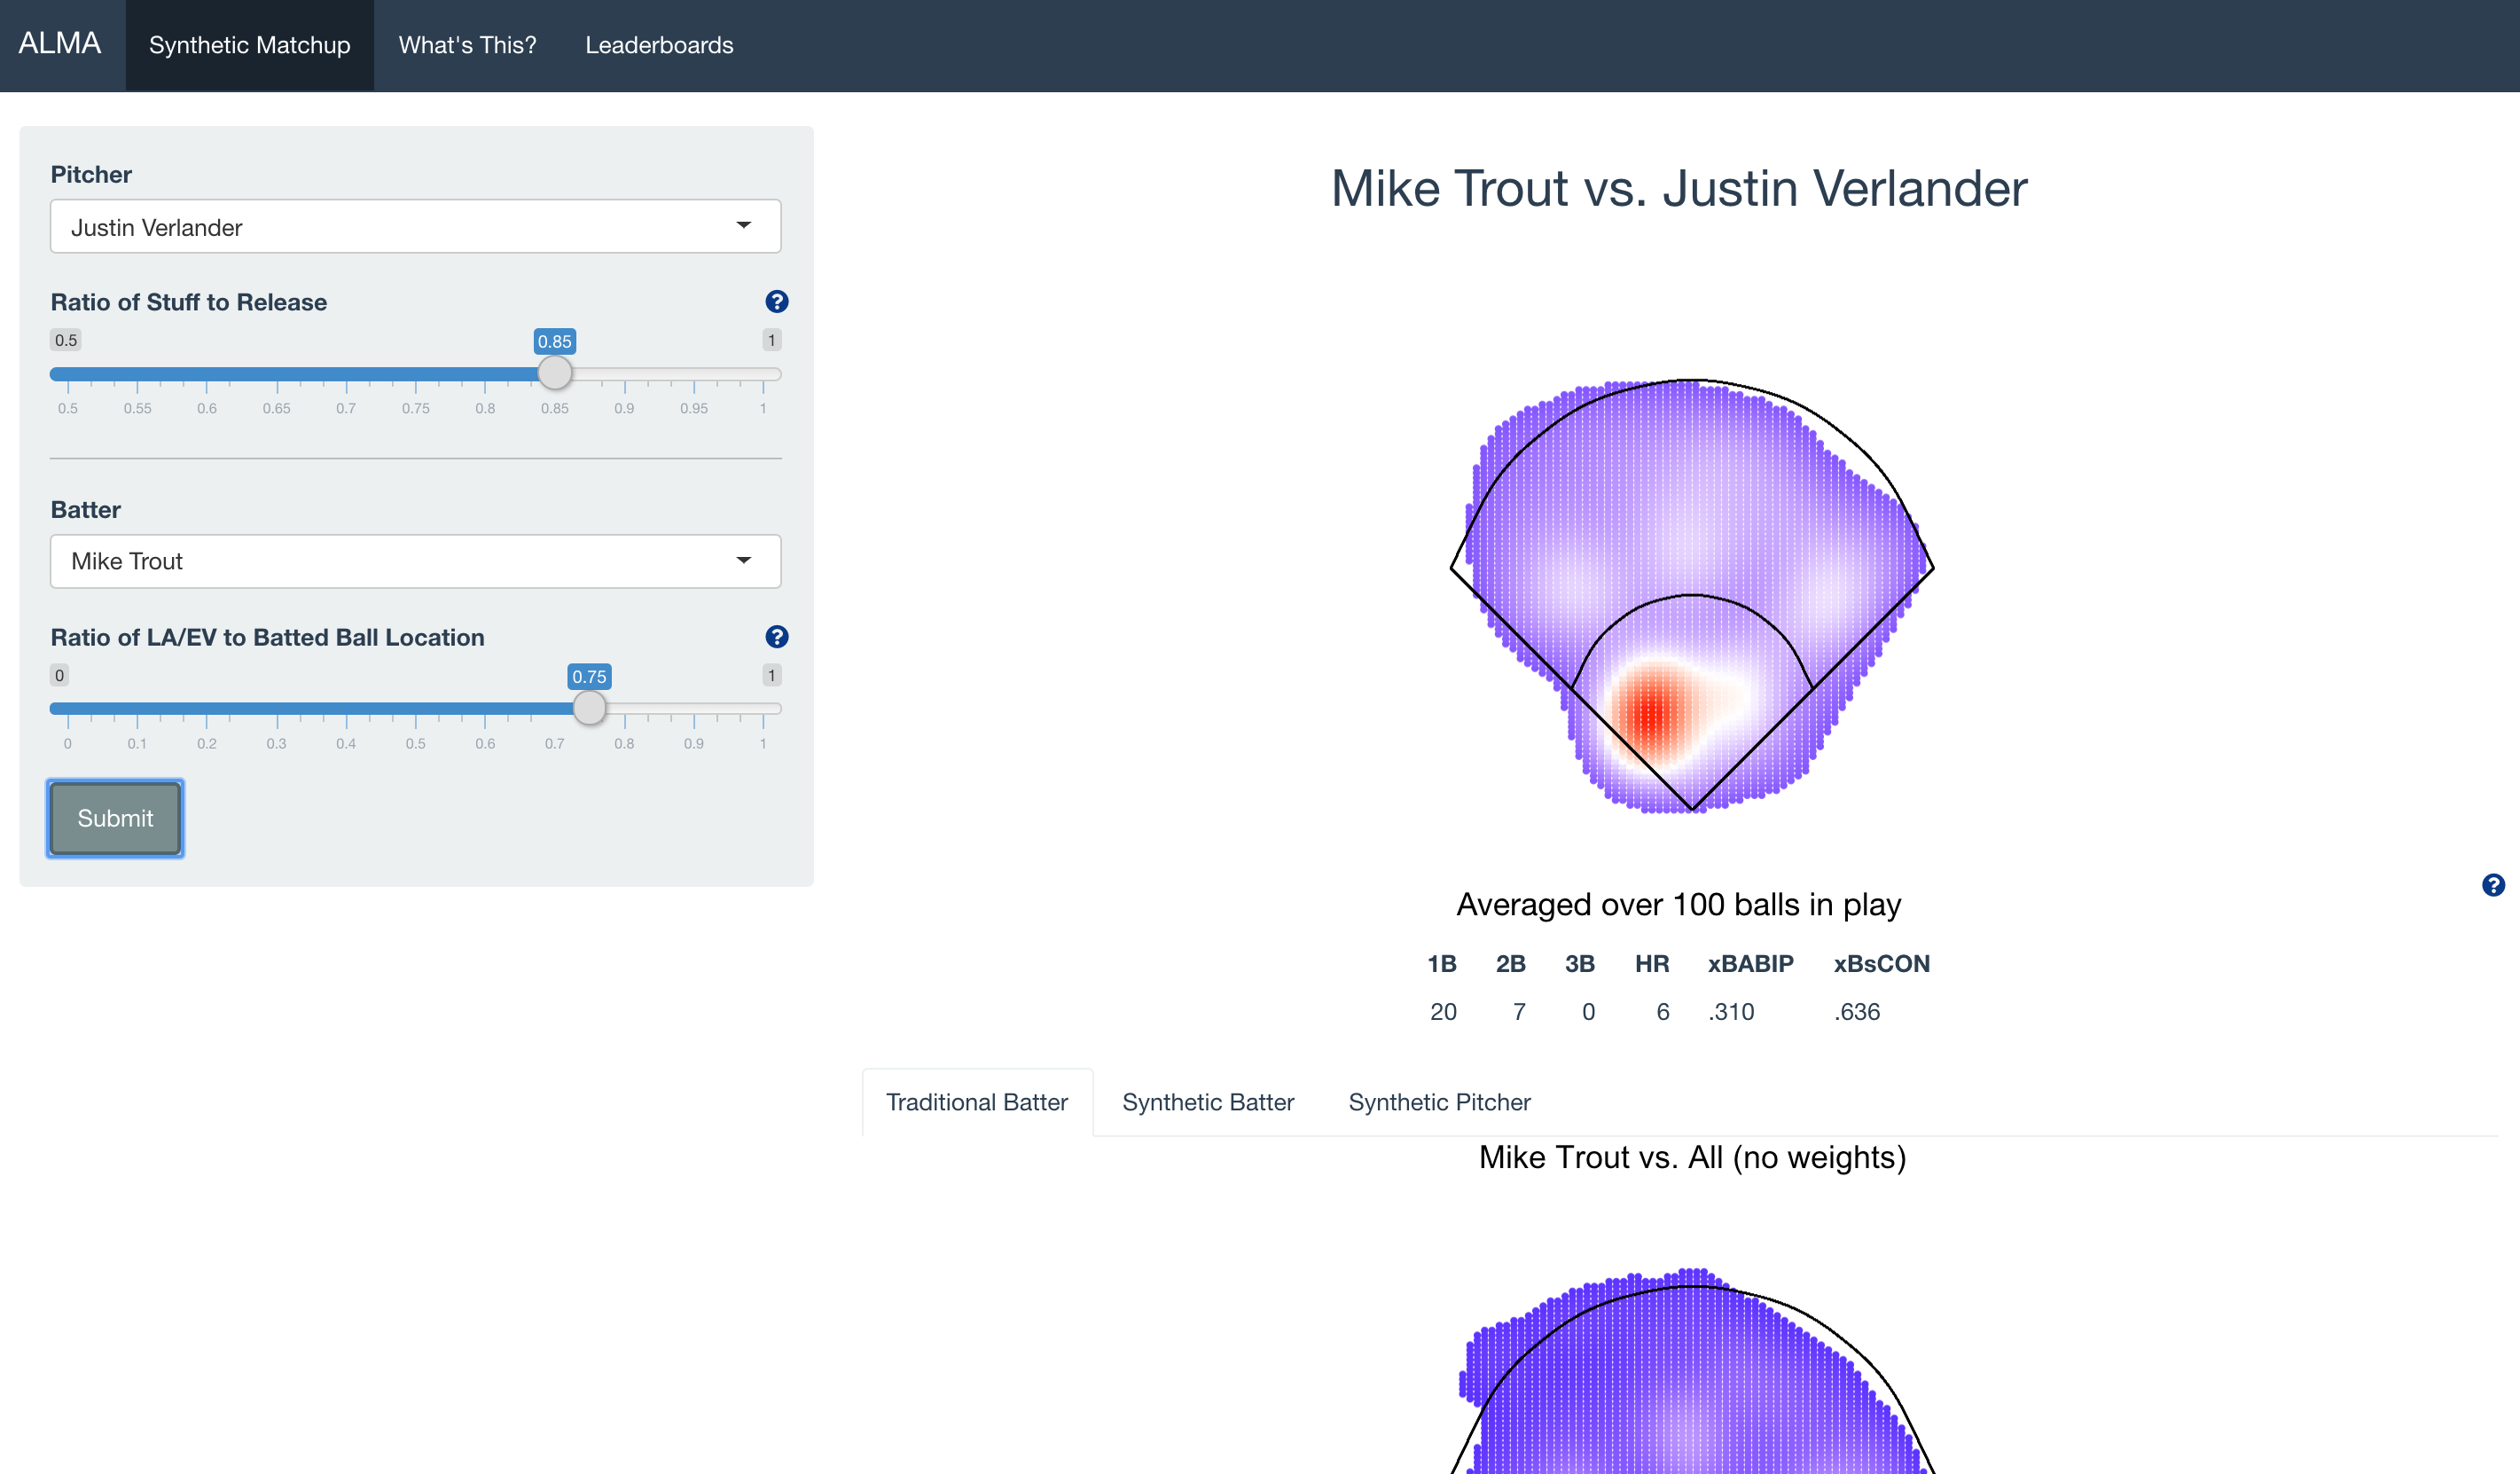
\includegraphics[width=5.5in, height=3in]{layout.png}
    \caption{The layout of the application upon submission.}
    \label{layout}
\end{figure}

\begin{figure}
\centering
\text{[Figure 2 about here]}
%    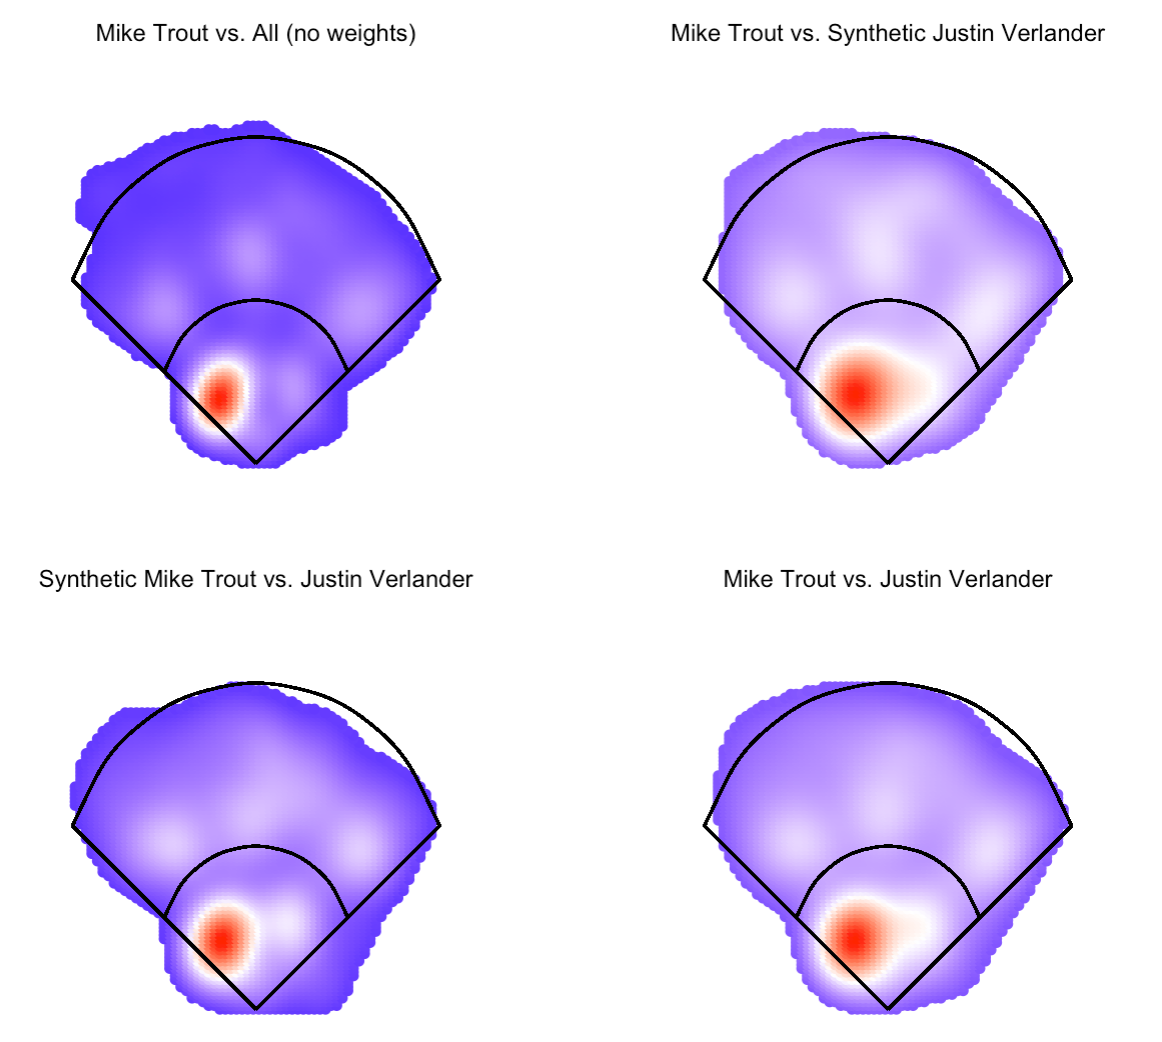
\includegraphics[width=4in, height=3in]{combined.png}  
    \caption{Spray chart distributions constructed by our app.  This example 
    corresponds to the spray chart distribution when batter Mike Trout faces 
    pitcher Justin Verlander.
    The top-left panel is the complete synthetic spray chart for 
      the batter-pitcher matchup.
    The top-right panel is the traditional batter-pitcher spray chart 
      distribution, with no consideration of similar players.
    The bottom-left panel is the synthetic batter's spray chart distribution 
      versus the real pitcher. 
    The bottom-right panel is the real batter's spray chart distribution 
      versus the synthetic batter.}
    \label{spraydists}
\end{figure}
%\begin{figure}
%\centering
%    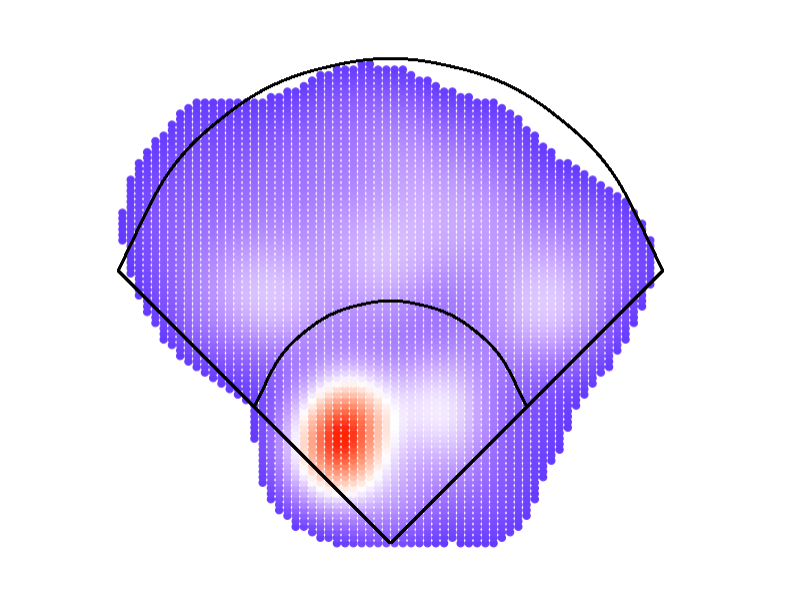
\includegraphics[width=3in, height=2in]{synthetic_trout.png}
%    \caption{Mike Trout's synthetic spray chart versus Justin Verlander}
%\end{figure}
%\begin{figure}
%\centering
%    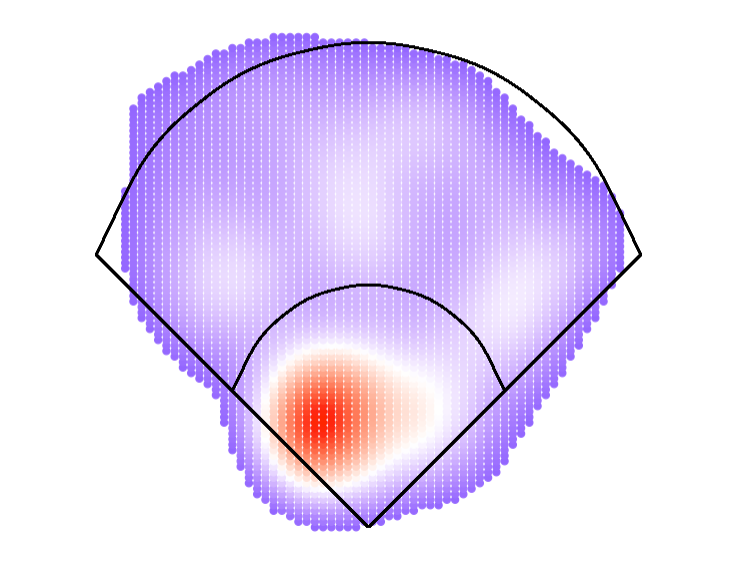
\includegraphics[width=3in, height=2in]{synthetic_verlander.png}
%    \caption{Justin Verlander's synthetic spray chart versus Mike Trout}
%\end{figure}
%\begin{figure}
%\centering
%    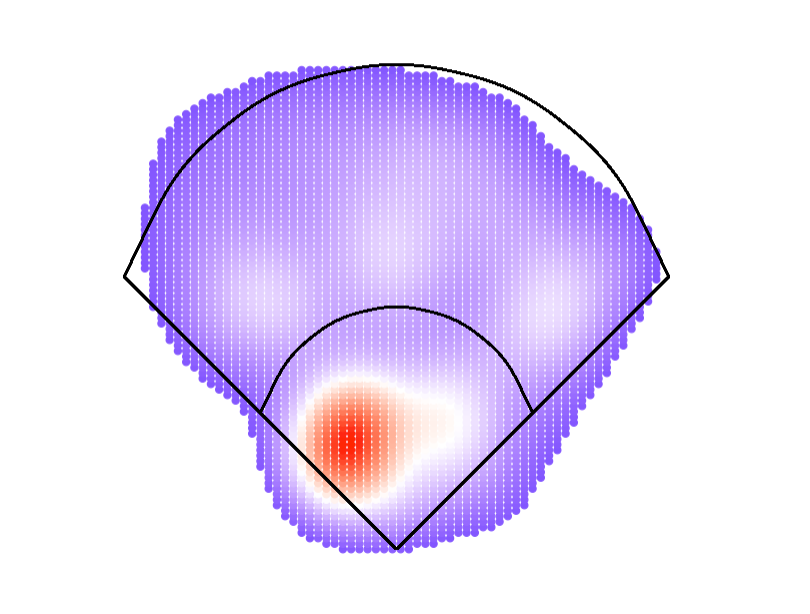
\includegraphics[width=3in, height=2in]{trout_verlander_master.png}
%    \caption{The complete synthetic spray chart for Mike Trout versus Justin Verlander}
%\end{figure}



%\noindent Some things to do:
%\begin{itemize}
%\item[1.] Find one or two interesting matchups. Include pictures of the display \\

%\item[2.] Explain what the sliders do and why they are important. \\
%One slider changes the ratio of pitcher “stuff” to release metrics. Stuff includes velocity, spin %rate, and movement. Release includes release angles and release point.
%One slider changes the ratio of batter launch conditions to location. Launch conditions includes %exit velocity and launch angle. Location includes pull\%, middle\%, oppo\%. These can be used to %tailor the comparisons - for example, it may be more useful to weight batted ball location higher %to alter infielder position, while it may be more useful to weight launch conditions higher to alter outfielder depth.

%\item[3.] Explain why these visualizations and metrics offer users. \\
%As mentioned above, these visualizations can help coaches position their fielders effectively. While a traditional spray chart may be useful in aggregate, building a custom spray chart to reflect a specific pitcher-batter matchup will yield more accurate results on a plate appearance by plate appearance level.

%\item[4.] Highlight that the Shiny app displays the most similar players. \\
%Below the two synthetic charts, there is a leaderboard displaying the most similar pitchers/batters. %These include their similarity and a variety of performance metrics.

%\end{itemize}

The pitcher slider allows users to determine the relative importance of ``stuff'', a colloquial term for pitch quality, versus release information. Stuff includes velocity, spin rate, and movement. Release includes release angles and release point. The batter slider allows users to determine the relative importance of launch conditions versus batted ball locations. Launch conditions includes exit velocity and launch angle. Location includes pull\%, middle\%, oppo\% (the percentage of batted balls place into the corresponding thirds of a baseball field). The default setting of the pitcher slider favors stuff over release information. The logic for this is quality of pitches being more representative of ability than release point. The default setting of the batter slider favors quality of contact over batted ball tendencies which appears to bias the synthetic batter's spray chart away from that of the batter under consideration. That being said, the batted ball tendencies are recorded as percentages of balls hit to six large grids on the baseball field, ignoring the quality, trajectory, and exact location of the batted ball. Thus, the quality of contact forms a more complete representation of a batter's skill than tendency.

As previously mentioned, these visualizations can help coaches position their fielders effectively. While a traditional spray chart may be useful in aggregate, building a custom spray chart to reflect a specific batter-pitcher matchup will yield more accurate results on a plate appearance by plate appearance level. This synthetically created spray chart will give the user an expected distribution of batted balls for the batter-pitcher matchup based on a combination of the distribution of similar batters against the pitcher, the distribution of similar pitchers against the batter, and the distribution of any observations of the pitcher vs batter since 2015. The app also displays two additional synthetic charts and a leaderboard displaying the most similar pitchers/batters. These include their overall similarity score and a variety of performance metrics. See Figure~\ref{synthpitcher} for an example of the top 10 most similar pitchers to Justin Verlander.

\begin{figure}
\centering
\text{[Figure 3 about here]}
    %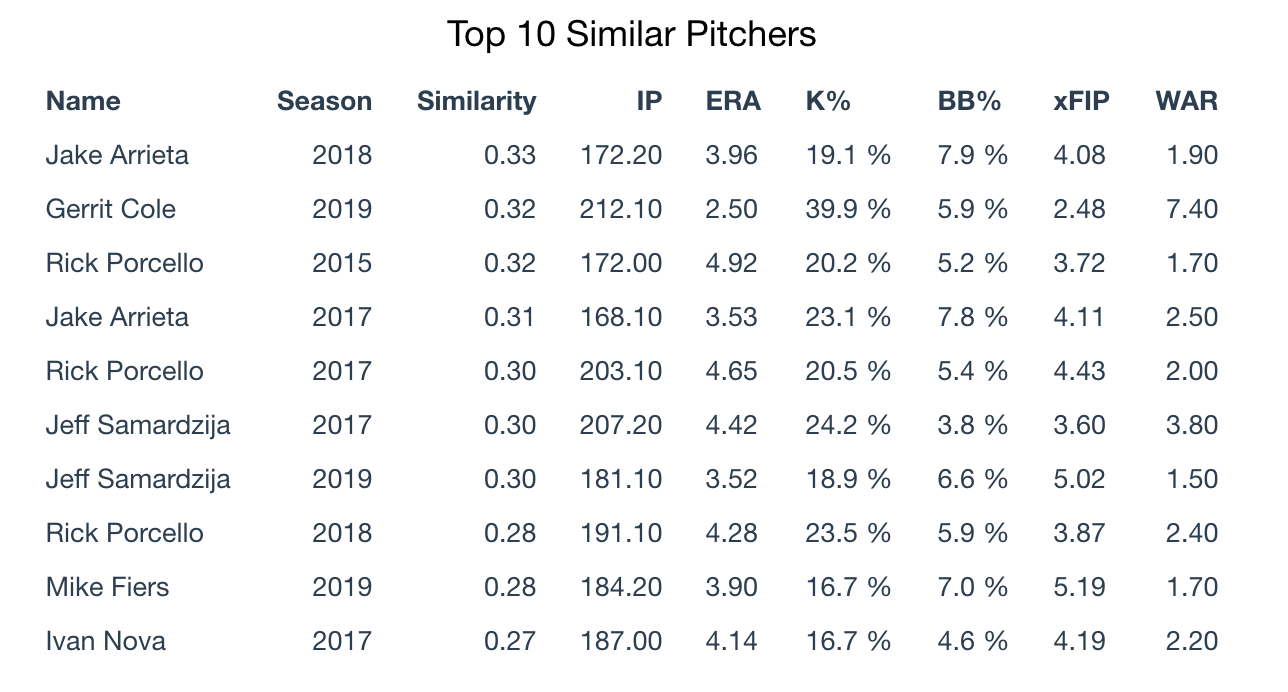
\includegraphics[width=6in, height=3in]{verlander_similar.png}
    \caption{The most similar pitchers to Justin Verlander with an 85\% stuff-to-release ratio}
    \label{synthpitcher}
\end{figure}

This matchup presents a good example of how to interpret the resulting spray charts. Trout seems to be a pull-heavy hitter in general according to his traditional chart. When facing pitchers similar to Verlander, he seems to push the ball the opposite way. This may be explained by Verlander's high velocity fastball. In general, batters have a hard time ``getting around'' (pulling) an upper-90's fastball, so they end up hitting the ball to the opposite field. Given this spray chart distribution, a coach may position the shortstop more towards third base, the second baseman more up the middle, and the first baseman more towards second base. This will protect against Trout's usual habit of pulling the ball, and also put the first baseman in a position to cover the opposite field soft ground ball. If this decision were made just by Trout's traditional chart, the first baseman might not have been moved to cover ground balls through the right side.





\section{Discussion}

The primary contribution of this work is the development of SEAM methodology in which a synthetic spray chart density function $\hat{g}_{\lambdabf}(\y|\x)$ is estimated. In our context of batter-pitcher matchups, this estimated density function is a weighted average of $f_\h(\y|\x)$, $\hat f_{\text{sp}}(\y|\x_p)$, and $\hat f_{\text{sb}}(\y|\x_b)$. The weights are chosen to minimize MSE under an assumed smooth function space. The synthetic players are constructed to best mimic the players under study. Our method of synthetic player construction is generalizable to other settings in baseball as well as other sports.

We also provide a Shiny app which implements SEAM methodology. This app provides users with visual and numeric summary measures of batter-pitcher matchups and it will be of interest to baseball fans, analysts, players, and team executives alike. Our application shows users batter tendencies versus pitchers while providing summaries of their overall success or lack thereof. Our application greatly improves upon the inferential power of spray charts \citep{pettispray, marchi2019analyzing} as a visualization of a batter's talent and hitting tendencies. Spray charts may be uninformative for individual matchups due to a lack of data. Our synthetic player construction alleviates this problem.

We are not the first to incorporate additional players into an analysis via similarity scores with the understanding that doing so improves estimation performance. The PECOTA prediction methodology \citep{PECOTA} tries to forecast the ability of players using aggregate estimates obtained from other similar players. To the best of our knowledge, we are the first to base similarity scores exclusively on Statcast data which we believe provides a truer notion of talent similarity.  




%\section*{Acknowledgements}

%We would like to thank ATLAS Infrastructure and Illini Analytics for computational resources that made our Shiny app possible. We would also like to thank Alan Nathan, Jim Albert, James Balamuta, Dootika Vats, John Marden, and Dave Zhao for helpful comments that improved our article and our Shiny app.


\section*{Appendix: Justification for our choice of $\lambdabf$}

We now motivate $\lambdabf$ theoretically. We first assume some additional structure on the space of functions that $f(\cdot|\cdot)$ belongs to in order to facilitate our motivation. The best batters in baseball are good at hitting the ball with general intent but batted ball locations will still exhibit variation. Therefore we expect spray chart densities to be smooth and lacking sharp peaks. It is reasonable to assume that $f(\cdot|\cdot)$ belongs to a multivariate H{\"o}lder class of densities which we will denote by $H(\beta,L)$. The space $H(\beta,L)$ is the set of functions $f(\y|\x)$ such that 
\begin{align*}
|D_{\y}^\s f(\y|\x) - D_{\y}^\s f(\y'|\x)| &\leq L_\x\|\y - \y'\|^{\beta - |\s|}, \\
|D_{\x}^\tbf f(\y|\x) - D_{\x}^\tbf f(\y|\x')| &\leq L_\y\|\x - \x'\|^{\beta - |\tbf|}, 
\end{align*}
for all $\y,\y' \in \Y$, all $\x,\x' \in \X$, and all $\s$ such that $|\s| = \beta - 1$ where
$D_{\y}^\s = \partial^{s_1 + s_2}/\partial y_1^{s_1} \partial y_2^{s_2}$, 
$D_{\x}^\tbf = \partial^{t_1 + \cdots + t_p}/\partial x_1^{t_1} \cdots \partial x_p^{t_p}$ and $L_\x \leq L$ for all $\x \in \X$ and $L_\y \leq L$ for all $\y \in \Y$. 
% Notes on multi var kde: https://bookdown.org/egarpor/NP-UC3M/kde-ii-asymp.html
We will assume the following regularity conditions for our spray chart distributions and kernel functions: 

\begin{itemize}
\item[A1.] The density $f$ is square integrable, twice continuously differentiable, and all the second order partial derivatives are square integrable. We will suppose that $\beta = 2$ in $H(\beta,L)$.
\item[A2.] The kernel $K$ is a spherically symmetric and bounded pdf with finite second moment and square integrable.
\item[A3.] $\Hbf = \Hbf_n$ is a deterministic sequence of positive definite symmetric matrices such that, $n\det(\Hbf) \to \infty$ when $n \to \infty$ and $\Hbf \to 0$ elementwise. 
\end{itemize}

Condition A2 holds for the multivariate Gaussian kernel function that we use in our implementation.
We will let $\Hbf$ be a matrix of bandwidth parameters that has diagonal elements $\h$, in our implementation $\Hbf = \text{diag}(\h)$. We will use the following notation: $R_{\x}(f) = \int f(\y|\x)^2 d\y$, $\mu_2(K) = \int u^2K(u)du$, and $\Hcal_f(\y|\x)$ is the Hessian matrix respect to $f(\y|\x)$ where derivatives are taken with respect to $\y$. Assume that pitch outcomes are independent across at bats and that $n_{p,j} = O(n)$, $n_{b,k} = O(n)$ and $\h_{p,j} = O(\h)$, $\h_{b,k} = O(\h)$ for all $j = 1, \ldots, J$, $k = 1, \ldots, K$. 

With the specification that $\beta = 2$ in Condition A1 we have that 
$
   f(\y|\x) - L\|\x-\x'\|^2 \leq f(\y|\x') \leq f(\y|\x) + L\|\x-\x'\|^2.
$
This result implies that
\begin{align*}
  R_{\x'}(f) - R_\x(f) &= \int (f(\y|\x')^2 - f(\y|\x)^2) d\y 
     = \int (f(\y|\x') - f(\y|\x))(f(\y|\x') + f(\y|\x)) d\y \\
  &\leq L\|\x'-\x\|^2 \int(f(\y|\x') + f(\y|\x)) d\y 
    = 2L\|\x'-\x\|^2,
\end{align*}
and 
$
   R_\x(f) - 2L\|\x-\x'\|^2 \leq R_{\x'}(f) \leq R_\x(f) + 2L\|\x-\x'\|^2.
$ 

We will define $\tilde \x_{b,k} = (\x_p',\x_{b,k}')'$ and $\tilde \x_{p,j} = (\x_{p,j}',\x_b')'$ for notational convenience, and will additionally assume the following regularity approximations:
\begin{itemize}
\item[A4.] The quantities $\sum_{j=1}^Jw_{p,j}^2\|\x - \tilde \x_{p,j}\|^m$ and $\sum_{k=1}^Kw_{b,k}^2\|\x - \tilde \x_{b,k}\|^m$ are negligible, where $m = 2,4$.
\item[A5.] The quantities $\sum_{j=1}^Jw_{p,j}\left(\h_{p,j}'\text{diag}(\Hcal_f(\y|\x_{p,j},\x_b))\h_{p,j} - \h'\text{diag}(\Hcal_f(\y|\x))\h\right)$ and \\$\sum_{k=1}^Kw_{b,k}\left(\h_{b,k}'\text{diag}(\Hcal_f(\y|\x_p,\x_{b,k}))\h_{b,k} - \h'\text{diag}(\Hcal_f(\y|\x))\h\right)$ are negligible.
\end{itemize}
Approximation A4 is reasonable in our baseball application where there are many players similar enough to the players under study so that $\sum_{j=1}^Js_{p,j} > 1$ and $\sum_{k=1}^Ks_{b,k} > 1$ and $s_{p,j}\|\x-\tilde\x_{p,j}\|^m, s_{b,k}\|\x-\tilde\x_{b,k}\|^m \to 0$ as $\|\x-\tilde\x_{p,j}\|,\|\x-\tilde\x_{b,k}\| \to \infty$ for all integers $m$. Approximation A5 is reasonable by similar logic. Specification of $\beta = 2$ implies that  
$\|\text{diag}(\Hcal_f(\y|\x_p,\x_{b,k})) - \text{diag}(\Hcal_f(\y|\x))\| \leq \sqrt{d_p}L$ and 
$\|\text{diag}(\Hcal_f(\y|\x_{p,j},\x_b)) - \text{diag}(\Hcal_f(\y|\x))\| \leq \sqrt{d_b}L$
where $d_p$ and $d_b$ are, respectively, the dimension of $\x_p$ and $\x_b$. 

%Properties to verify
%$$
%  \E(\hat f_\h(\y|\x)) - f(\y|\x) \approx \frac{\mu_2(K)\h'\Hcal_f(\y|\x)\h}{2}
%$$
%and
%$$
% \Var(\hat f_\h(\y|\x)) \approx \frac{R_{\x}(f)f(\y|\x)}{\det(\Hbf)}
%$$

% https://www.ssc.wisc.edu/~bhansen/718/NonParametrics1.pdf
%From Hansen's notes: 

We now have enough structure to estimate the MSE of \eqref{spraydens} and \eqref{sd-implem}. Standard results from nonparametric estimation theory give
$$
  \E(\hat f_\h(\y|\x)) - f(\y|\x) = \frac{\mu_2(K)\h'\text{diag}(\Hcal_f(\y|\x))\h}{2} 
    + o(\|\h\|^2),
$$
and
$$
 \Var(\hat f_\h(\y|\x)) = \frac{R_{\x}(f)f(\y|\x)}{n\det(\Hbf)} + O\left(\frac{1}{n}\right).
$$

Our multivariate H{\"o}lder class specifications yield,
\begin{align*}
  &\E(\hat g_{\lambdabf}(y|x)) = \lambda \E \hat f_\h(\y|\x)
    + \lambda_p \E \hat f_{\text{sp}}(\y|\x_b) 
    + \lambda_b \E \hat f_{\text{sb}}(\y|\x_p) \\
  &\qquad= \lambda f(\y|\x) +  \lambda \frac{\mu_2(K)\h'\text{diag}(\Hcal_f(\y|\x))\h}{2} 
    + \lambda_p \sum_{j=1}^J w_{p,j} \E \hat f_{\h_{p,j}}(\y|\x_{p,j},\x_b) \\
    &\qquad\qquad+ \lambda_b \sum_{k=1}^K w_{b,k} \E \hat f_{\h_{b,k}}(\y|\x_p,\x_{b,k}) 
    + o(\|\h\|^2) \\
  &\qquad= \lambda f(\y|\x) +  \lambda \frac{\mu_2(K)\h'\text{diag}(\Hcal_f(\y|\x))\h}{2} 
  + o(\|\h\|^2) \\
    &\qquad\qquad+ \lambda_p \sum_{j=1}^J w_{p,j} f_{\h_{p,j}}(\y|\x_{p,j},\x_b) 
      + \lambda_p\sum_{j=1}^Jw_{p,j}
      \frac{\mu_2(K)\h_{p,j}'\text{diag}(\Hcal_f(\y|\x_{p,j},\x_b))\h_{p,j}}{2} \\
    &\qquad\qquad+ \lambda_b \sum_{k=1}^K w_{b,k} f_{\h_{b,k}}(\y|\x_p,\x_{b,k}) 
      + \lambda_b\sum_{k=1}^K w_{b,k}
      \frac{\mu_2(K)\h_{b,k}'\text{diag}(\Hcal_f(\y|\x_p,\x_{b,k}))\h_{b,k}}{2},
\end{align*}
and 
\begin{align*}
  &\Var(\hat g_{\lambdabf}(y|x)) = \Var\left(\lambda \hat f_\h(\y|\x) 
    + \lambda_p \hat f_{\text{sp}}(\y|\x_b) 
    + \lambda_b \hat f_{\text{sb}}(\y|\x_p)\right) \\
  &= \lambda^2 \frac{R_{\x}(f)f(\y|\x)}{n\det(\Hbf)} + O\left(\frac{1}{n}\right)
    + \lambda_p^2 \sum_{j=1}^J w_{p,j}^2 \Var \hat f_{\h_{p,j}}(\y|\x_{p,j},\x_b) 
    + \lambda_b^2 \sum_{k=1}^K w_{b,k}^2 \Var \hat f_{\h_{b,k}}(\y|\x_p,\x_{b,k}) \\
  &= \lambda^2 \frac{R_{\x}(f)f(\y|\x)}{n\det(\Hbf)} + O\left(\frac{1}{n}\right)
    + \lambda_p^2 \sum_{j=1}^J w_{p,j}^2
      \frac{R_{\tilde \x_{p,j}}(f)f(\y|\x_{p,j},\x_b)}{n_{p,j}\det(\Hbf_{p,j})} 
    + \lambda_b^2 \sum_{k=1}^K w_{b,k}^2
      \frac{R_{\tilde\x_{b,k}}(f)f(\y|\x_p,\x_{b,k})}{n_{b,k}\det(\Hbf_{b,k})},
\end{align*}
Let $\theta_{p,j} = n\det(\Hbf)/n_{p,j}\det(\Hbf_{p,j})$ and $\theta_{b,k} = n\det(\Hbf)/n_{b,k}\det(\Hbf_{b,k})$. With these specifications, we have that
\begin{align*}
  &\Var(\hat g_{\lambdabf}(y|x)) - \Var(\hat f_\h(\y|\x)) + O\left(\frac{1}{n}\right) \\
  &=(\lambda^2 - 1)\frac{R_{\x}(f)f(\y|\x)}{n\det(\Hbf)} 
    + \lambda_p^2 \sum_{j=1}^J \theta_{p,j}w_{p,j}^2
      \frac{R_{\tilde \x_{p,j}}(f)f(\y|\x_{p,j},\x_b)}{n\det(\Hbf)} 
    + \lambda_b^2 \sum_{k=1}^K \theta_{b,k}w_{b,k}^2 
      \frac{R_{\tilde\x_{b,k}}(f)f(\y|\x_p,\x_{b,k})}{n\det(\Hbf)} \\
  &\leq \left(\lambda^2 + \lambda_p^2 \sum_{j=1}^J \theta_{p,j}w_{p,j}^2
    + \lambda_b^2 \sum_{k=1}^K \theta_{b,k}w_{b,k}^2 - 1\right)
      \frac{R_{\x}(f)f(\y|\x)}{n\det(\Hbf)} \\
    &\qquad\qquad+ \lambda_p^2 \sum_{j=1}^J \theta_{p,j}w_{p,j}^2
      \left(\frac{R_{\x}(f)\|\x-\tilde \x_{p,j}\|^2 
      + 2Lf(\y|\x)\|\x-\tilde \x_{p,j}\|^2 + 2L^2\|\x-\tilde \x_{p,j}\|^4}{n\det(\Hbf)}\right) \\
    &\qquad\qquad+ \lambda_b^2 \sum_{k=1}^K \theta_{b,k}w_{b,k}^2
      \left(\frac{R_{\x}(f)\|\x-\tilde \x_{b,k}\|^2 
      + 2Lf(\y|\x)\|\x-\tilde \x_{b,k}\|^2 + 2L^2\|\x-\tilde \x_{b,k}\|^4}{n\det(\Hbf)}\right).
\end{align*}
Our assumption on the $w_{b,k}^2\|\x-\tilde \x_{,k}\|^m$ and $w_{p,j}^2\|\x-\tilde \x_{p,j}\|^m$, for $m = 2,4$, and an identical lower bound argument implies that 
$$
  \Var(\hat g_{\lambdabf}(y|x)) - \Var(\hat f_\h(\y|\x)) 
    \approx \left(\lambda^2 + \lambda_p^2 \sum_{j=1}^J\theta_{p,j}w_{p,j}^2 
      + \lambda_b^2 \sum_{k=1}^K \theta_{b,k}w_{b,k}^2 - 1\right)
      \frac{R_{\x}(f)f(\y|\x)}{n\det(\Hbf)} + O\left(\frac{1}{n}\right).
$$
We also have
\begin{align*}
  \text{Bias}(\hat f_\h(\y|\x),f(\y|\x))^2 
    &= \left(\frac{\mu_2(K)\h'\text{diag}(\Hcal_f(\y|\x))\h}{2} 
    + o(\|\h\|^2)\right)^2,
\end{align*}
and regularity approximations A4 and A5 yield
\begin{align*}
  &\text{Bias}(\hat g_{\lambdabf}(\y|\x),f(\y|\x))^2 = \left(\lambda f(\y|\x) - f(\y|\x) 
    +  \lambda \frac{\mu_2(K)\h'\text{diag}(\Hcal_f(\y|\x))\h}{2} + o(\|\h\|^2)\right. \\
    &\qquad+ \lambda_p \sum_{j=1}^J w_{p,j} f(\y|\x_{p,j},\x_b) 
      + \lambda_p\sum_{j=1}^Jw_{p,j}
      \frac{\mu_2(K)\h_{p,j}'\text{diag}(\Hcal_f(\y|\x_{p,j},\x_b))\h_{p,j}}{2} \\
    &\qquad+ \left.\lambda_b \sum_{k=1}^K w_{b,k} f(\y|\x_p,\x_{b,k}) 
      + \lambda_b\sum_{k=1}^K w_{b,k}
      \frac{\mu_2(K)\h_{b,k}'\text{diag}(\Hcal_f(\y|\x_p,\x_{b,k}))\h_{b,k}}{2}\right)^2 \\
 &\leq \left(\lambda f(\y|\x) - f(\y|\x) 
    +  \lambda \frac{\mu_2(K)\h'\text{diag}(\Hcal_f(\y|\x))\h}{2} + o(\|\h\|^2)\right. \\
    &\qquad+ \lambda_p \sum_{j=1}^J w_{p,j}(f(\y|\x) + L(-1)^t\|\x - \tilde\x_{p,j}\|^2)
      + \lambda_p\sum_{j=1}^Jw_{p,j}\frac{\mu_2(K)\h'\text{diag}(\Hcal_f(\y|\x))\h}{2} \\  
    &\qquad+ \left.\lambda_b \sum_{k=1}^K w_{b,k}(f(\y|\x) 
      + L(-1)^t\|\x - \tilde\x_{b,k}\|^2)
      + \lambda_b\sum_{k=1}^K w_{b,k}\frac{\mu_2(K)\h'\text{diag}(\Hcal_f(\y|\x))\h}{2}\right)^2 \\
 &\approx \left(\lambda_p \sum_{j=1}^J (-1)^t Lw_{p,j}\|\x - \tilde\x_{p,j}\|^2 
   + \lambda_b \sum_{k=1}^K (-1)^tLw_{b,k}\|\x - \tilde\x_{b,k}\|^2\right. \\
   &\qquad+ \left.\frac{\mu_2(K)\h'\text{diag}(\Hcal_f(\y|\x))\h}{2} + o(\|\h\|^2)\right)^2,
\end{align*}
where $t \in \{0,1\}$ is chosen to satisfy the above inequality. Putting these variance and bias results together without the lower order terms yields
\begin{align*}
  &MSE(\hat g_{\lambdabf}(\y|\x),f(\y|\x)) - MSE(\hat f_{\h}(\y|\x),f(\y|\x)) \\
    &\qquad\leq \left(\lambda^2 + \lambda_p^2 \sum_{j=1}^J\theta_{p,j}w_{p,j}^2 
      + \lambda_b^2 \sum_{k=1}^K \theta_{b,k}w_{b,k}^2 - 1\right)
      \frac{R_{\x}(f)f(\y|\x)}{n\det(\Hbf)} \\
    &\qquad+ \left(\lambda_p \sum_{j=1}^J (-1)^t Lw_{p,j}\|\x - \tilde\x_{p,j}\|^2 
     + \lambda_b \sum_{k=1}^K (-1)^tLw_{b,k}\|\x - \tilde\x_{b,k}\|^2 + 
     \frac{\mu_2(K)\h'\text{diag}(\Hcal_f(\y|\x))\h}{2}\right)^2 \\
    &\qquad- \left(\frac{\mu_2(K)\h'\text{diag}(\Hcal_f(\y|\x))\h}{2}\right)^2.
\end{align*}
This motivates the following choice of $\lambdabf$,
$$
  \lambda = \frac{\sqrt{n}}{\sqrt{n} + \sqrt{n_p} + \sqrt{n_b}}, \qquad
  \lambda_p = \frac{\sqrt{n_p}}{\sqrt{n} + \sqrt{n_p} + \sqrt{n_b}}, \qquad
  \lambda_b = \frac{\sqrt{n_b}}{\sqrt{n} + \sqrt{n_p} + \sqrt{n_b}},
$$
where $n_p = \sum_{j=1}^J s_{p,j}^2n_{p,j}$ and $n_b = \sum_{k=1}^K s_{b,k}^2n_{b,k}$. We will now develop intuition for these choices. First, notice that $\lambda_p,\lambda_b \to 0$ as 
$\min_j(\|\x - \tilde\x_{p,j}\|), \min_k(\|\x - \tilde\x_{b,k}\|) \to \infty$. These cases correspond, to there being no similar pitchers or batters to the players under study. We turn attention to the bias terms, notice that 
$$
  \lambda_p\sum_{j=1}^J (-1)^t Lw_{p,j}\|\x - \tilde\x_{p,j}\|^2 
    = \frac{\sqrt{\sum_{j=1}^J s_{p,j}^2n_{p,j}}
      \sum_{j=1}^J (-1)^t Lw_{p,j}\|\x - \tilde\x_{p,j}\|^2}
      {\sqrt{n} + \sqrt{n_p} + \sqrt{n_b}} \longrightarrow 0,
$$
when there exists some $j'$ such that $\|\x - \tilde\x_{p,j}\| \to 0$ or $\min_j(\|\x - \tilde\x_{p,j}\|) \to \infty$. These cases correspond, respectively, to there being a few highly similar pitchers or there being no similar pitchers to the pitcher under study. Thus, the discrepancy in bias vanishes in the extreme cases. The same argument holds for batters. Now notice that
$$
  \lambda_p^2 \sum_{j=1}^J\theta_{p,j}w_{p,j}^2 
    = \frac{\sum_{j=1}^J s_{p,j}^2n_{p,j}\sum_{j=1}^J\theta_{p,j}w_{p,j}^2}
      {(\sqrt{n} + \sqrt{n_p} + \sqrt{n_b})^2} \longrightarrow 
      \left\{\begin{array}{cl}
       0, & \min_j(\|\x - \tilde\x_{p,j}\|) \to \infty; \\
         & \\
       \frac{n}
         {(\sqrt{n} + \sqrt{n_{p,j'}} + \sqrt{n_b})^2}, & w_{p,j'} \to 1.
      \end{array}\right.
$$
The same argument holds for batters. Therefore, when there is a pitcher $j'$ and batter $k'$ so that  $w_{p,j'},w_{b,k'} \to 1$, we have that 
$$
  \left(\lambda^2 + \lambda_p^2 \sum_{j=1}^J \theta_{p,j}w_{p,j}^2
    + \lambda_b^2 \sum_{k=1}^K \theta_{b,k}w_{b,k}^2 - 1\right) \longrightarrow 
    \frac{3n}
      {(\sqrt{n} + \sqrt{n_{p,j'}} + \sqrt{n_{b,k'}})^2} - 1.
$$
The above is not always less than 0 for all configurations. However, it will be less than 0 when $n$ is comparable to $n_{p,j'}$ and $n_{b,k'}$, a setting that we will guard against in our implementation by specifying a minimal sample size to enter into available player pool.


\bibliographystyle{chicago}
\bibliography{spray}


\end{document}

